\documentclass[preprint,12pt,authoryear]{elsarticle}
%\documentclass[final,1p,times,twocolumn,authoryear]{elsarticle}
\usepackage{lineno,hyperref}
\usepackage{fixltx2e}
\modulolinenumbers[5]

\journal{Geoderma}

%%%%%%%%%%%%%%%%%%%%%%%
%% Elsevier bibliography styles
%%%%%%%%%%%%%%%%%%%%%%%
%% To change the style, put a % in front of the second line of the current style and
%% remove the % from the second line of the style you would like to use.
%%%%%%%%%%%%%%%%%%%%%%%

%% Numbered
%\bibliographystyle{model1-num-names}

%% Numbered without titles
%\bibliographystyle{model1a-num-names}

%% Harvard
\bibliographystyle{model2-names.bst}\biboptions{authoryear}

%% Vancouver numbered
%\usepackage{numcompress}\bibliographystyle{model3-num-names}

%% Vancouver name/year
%\usepackage{numcompress}\bibliographystyle{model4-names}\biboptions{authoryear}

%% APA style
%\bibliographystyle{model5-names}\biboptions{authoryear}

%% AMA style
%\usepackage{numcompress}\bibliographystyle{model6-num-names}

%% `Elsevier LaTeX' style
%\bibliographystyle{elsarticle-harv}
%%%%%%%%%%%%%%%%%%%%%%%

\begin{document}

\begin{frontmatter}

\title{Topographic control on soil function evaluation -  a case study from South Tyrol}


%% Group authors per affiliation:

\author[mymainadress]{Fabian E. Gruber\corref{mycorrespondingauthor}}
\cortext[mycorrespondingauthor]{Corresponding author}
\ead{Fabian.Gruber@uibk.ac.at}
\author[mymainadress]{Jasmin Baruck}
\author[mymainadress]{Clemens Geitner}



\address[mymainadress]{Institute of Geography, University of Innsbruck, Innrain 52f, 6020 Innsbruck, Austria}

\begin{abstract}

\end{abstract}

\begin{keyword}
soil function evaluation, Alpine environment
\end{keyword}

\end{frontmatter}

\linenumbers

\section{Introduction}
Information on soil, a, at least from a human time perspective, non-renewable ressource, is of increasing importance given erosion, soil degradation and soil sealing. It is necessary to know where and where not certain practises are applicable and to adjust land-use planning appropriately. Accordingly, soil function evaluation is an invaluable tool for the future.\newline

\cite{Haslmayr2016} and further literature
\newline

In this study, we present the soil evaluation tool \emph{Soil Evaluation for Planning Procedures (SEPP)} and investigate topographic and parent material control of the different soil functions by applying a cross-validated machine learning approach based on availible soil pit information in the Oltradige/\"{U}beretsch region of the Autonomous Province Bolzano - South Tyrol.
\section{Data and methods}

\subsection{Study area and soil data}

\subsection{SEPP - Soil Evaluation for Planning Procedures}
The software SEPP currently computes a soil function evaluation based on soil pit descriptions. It requires that the pit descriptions are performed following the Austrian Soil classification  \citep{Nestroy2000,Nestroy2011} and related mapping manuals. The minimum  soil profile site characteristics are local slope, thickness of organic horizons, soil depth, groundwater table, soil parent material, soil type, humus form, altitudinal zone, moisture level and land use.For each horizon, the minimum characteristics necessary for computing the soil function are the master horizon designation, depth, pH value, proportion of the dominant soil structure type and class membership with regard to carbonate content, soil texture, organic content, abundance of rock fragments, bulk density, soil structure. These class attributes can be substituted by exact values if available. The soil functions, for which 15 different potentials are computed, are  \emph{habitat for living organisms} (specifically the potential as habitat for drought-tolerant species, moisture tolerant species, soil organisms and crops),  \emph{infiltration and drainage regulation} (minimum, average and heavy precipitation retention capacity as well as groundwater reformation rate), \emph{natural soil fertility} as well as \emph{filter and buffer for pollutants} (heavy metal, organic, acidifying and water-soluble). The result is a grade between 1 and 5 for each soil function potential, with 1 signifying a high potential and 5 a low one.

\paragraph{Potential as a habitat for drought-tolerant species} 
Both this potential and the following potential as a habitat for moisture-tolerant species are performed based on modifications of the approaches decribed by \cite{BAYGLA2003} and \cite{Lehmann2008}.
The evaluation of a soil's potential  as a habitat for drought-tolerant species is based on the parameters land use, soil type and available field capacity. While the first two parameters are applied to distinguish especially suited (ruderal locations and corresponding soil types) or unsuited (mire deposits and soil types commonly found on these) sites, the latter is used to grade those soil profile sites showing the remaining landuse and soil type combinations. 
\paragraph{Potential as a habitat for moisture-tolerant species}
This potential is evaluated similarly to the the one for drought-tolerant species, in that specific soil types, e.g. Gleysols, are attributed specific grades. In addition, the depth of the groundwater table is used to distinguish sites with high potential, and the available field capacity is used to differentiate even further.
\paragraph{Habitat for soil organisms}
This potential is evaluated according to \cite{Beylich2005} with some minor adaptions. In this framework, a number of species groups are used as indicators for the composition of soil life, with emphasis on earth worms (Lumbricidae) as they are influential on soil structure and bioturbation. This method is based on the relationship between soil organism communities and a number of abiotic soil parameters. Specifically, one of 14 possible soil organism communities, which are the basis for the grade awarded to a site, is attributed to a site according to a classification tree applying the parameters pH, moisture level, land use and soil texture.
\paragraph{Potential for agricultural production}
The assessment of the potential for agricultural production is performed according to the method proposed in the framework TUSEC-IP \citep{Lehmann2008} by an accumulative rating of five criteria. The criteria \emph{general conditions of the profile site} is rated based on soil depth, topsoil aggregate structure and topsoil as well as subsoil bulk density. While the criteria \emph{water supply} is based on available field capacity and the depth of the groundwater table, the grade for \emph{air supply} is derived from air capacity and for \emph{nutrient supply} the alkaline cation exchange capacity is regarded. The \emph{climate} criteria is derived from the mean annual temperature of the growing season if available, or else replaced by proxy values such as mean annual temperature or altitudinal zone. The combination of the grades of the individual criteria for agricultural production leads to an overall grade that is then adjusted for the slope gradient of the location.
\paragraph{Average and minimum precipitation retention capacity}
Following a modified version of the procedures presented by \cite{LUBW1995} and \cite{BAYGLA2003}, this potential is assessed by combining the permeability coefficient (using either the average value of the soil profile or the minimum value) with the water storage capacity. For more or less planar areas, the water storage capacity is regarded as  the sum of the usable field capacity and the air capacity, whereas for steeper slopes only the former parameter is used. Additionally, permeability coefficient and water storage capacity is considered only for soil horizons not linked to contact with groundwater or stagnant water.
\paragraph{Retention capacity for heavy precipitation events}
 The evaluation of this soil potential is a modfied version of the scheme proposed by \citep{Lehmann2008}. It differs from the agerage precipitation retention capacity by being based on the assumption that flooding hazards are greatest when soils are already saturated with water, and therefore only the air storage capacity is considered for retention. This retention volume is then compared to the design rainfall event under consideration of the infiltration rate.
\paragraph{Quality of groundwater reformation}
Also following \citep{Lehmann2008}, this potential is assessed using the same parameters as the precipitation capacity but considers the assumption that very quick infiltration leads to an increase of pollutants in the groundwater. In the same reasoning, soil types linked to groundwater or locations with high groundwater table are given poorer grades.
\paragraph{Potential for providing nutrients for plants}
Adhering to \citep{Mueller2011}, the assessment of this potential uses the parameter alkaline cation exchange capacity. As this is only a coarse approximation, this potential is not differentiated into five, but only three classes (poor, average and high potential).
\paragraph{Potential as a CO\textsubscript{2} sink}
By applying a modified version of the rating proposed by \cite{Gerstenberg2005}, selected land uses, especially forests, are awarded good grades, whereas other landuses are graded based on the amount of organic matter, summed up over all soil horizons.
\paragraph{Potential for retention of heavy metals}
In this assessment, the ability to bind cadmium is used as a proxy for other heavy metals. Based on modifications of the procedures proposed by \cite{AGBoden2000} and \cite{BAYGLA2003},in a first step this ability is evaluated for different pH-values for sandy soils with little organic content, and later adjusted with regard to organic matter content and soil texture as a proxy for clay content.
\paragraph{Potential for transforming organic contaminants}
As organic pollutants are generally transformed by soil organisms, this potential can be essentially assessed by rating the living conditions for soil micro-organisms. Consequently, the parameters which contribute to the rating procedure based on \cite{LUBW1995}  are topsoil organic matter content, topsoil clay content and the average topsoil pH-value. In a first step, microbial activity is estimated based on humus form and pH-value, and then the potential for transformation is further differentiated based on organic matter and clay content.
\paragraph{Potential as  filter and buffer for organic contaminants}
As the evaluation of a representative contaminant (such as cadmium for heavy metals) is not feasible for organic contaminants due to their variety, this potential is assessed by estimating a mean binding capacity for organic pollutants using organic matter and clay content for the fine material contained within a soil profile.
\paragraph{Potential for retention of water-soluble contaminants}
For the assessment of the potential for retention of water-soluble pollutants, with emphasis on nitrate, the yearly seepage rate is calculated based on mean precipitation, mean evaporation and an estimate of surface run-off derived from soil texture. The grade for this potential is rewarded based on the annual exchange rate of soil water by comparing seepage volume with field capacity.
\paragraph{Potential as buffer for acidic contaminants}
The potential buffer capacity is evaluated according to \cite{BAYGLA2003} by considering the alkaline cation exchange capacity and the carbonate content of the mineral horizons on the one hand, and estimating the buffer capacity of the organic layer from its humus form and thickness on the other hand.
\subsection{Variable selection procedure}
Support vector machine (SVM) classification is a statistical learning approach first described by \cite{Cortes1995}.
A forward step-wise feature selection procedure based on 10-fold cross-validation was applied to selection the best parameter or parameter combination for each soil function or potential. Cross-validation was also applied to the entire feature selection procedure. As the selection process sometime revealed a number of parameter combinations leading to comparable cross-validated accuracies, these were then compared by performing the 10-fold CV 100 times, each time with 10 different, random partitions. The median values and distribution of accuracy values were compared, as were the confusion matrixes based on the whole data set, where the final modelled soil function classes were attributed using the majority vote of the 100 predictions.

\section{Results}
The soil function grades for each of the 15 potentials was calculated for each of the 108 soil profile pits in the study area with the SEPP app. Figure \ref{fig:SFdistro} shows the distribution of these grades.
 \begin{figure}[ht!]
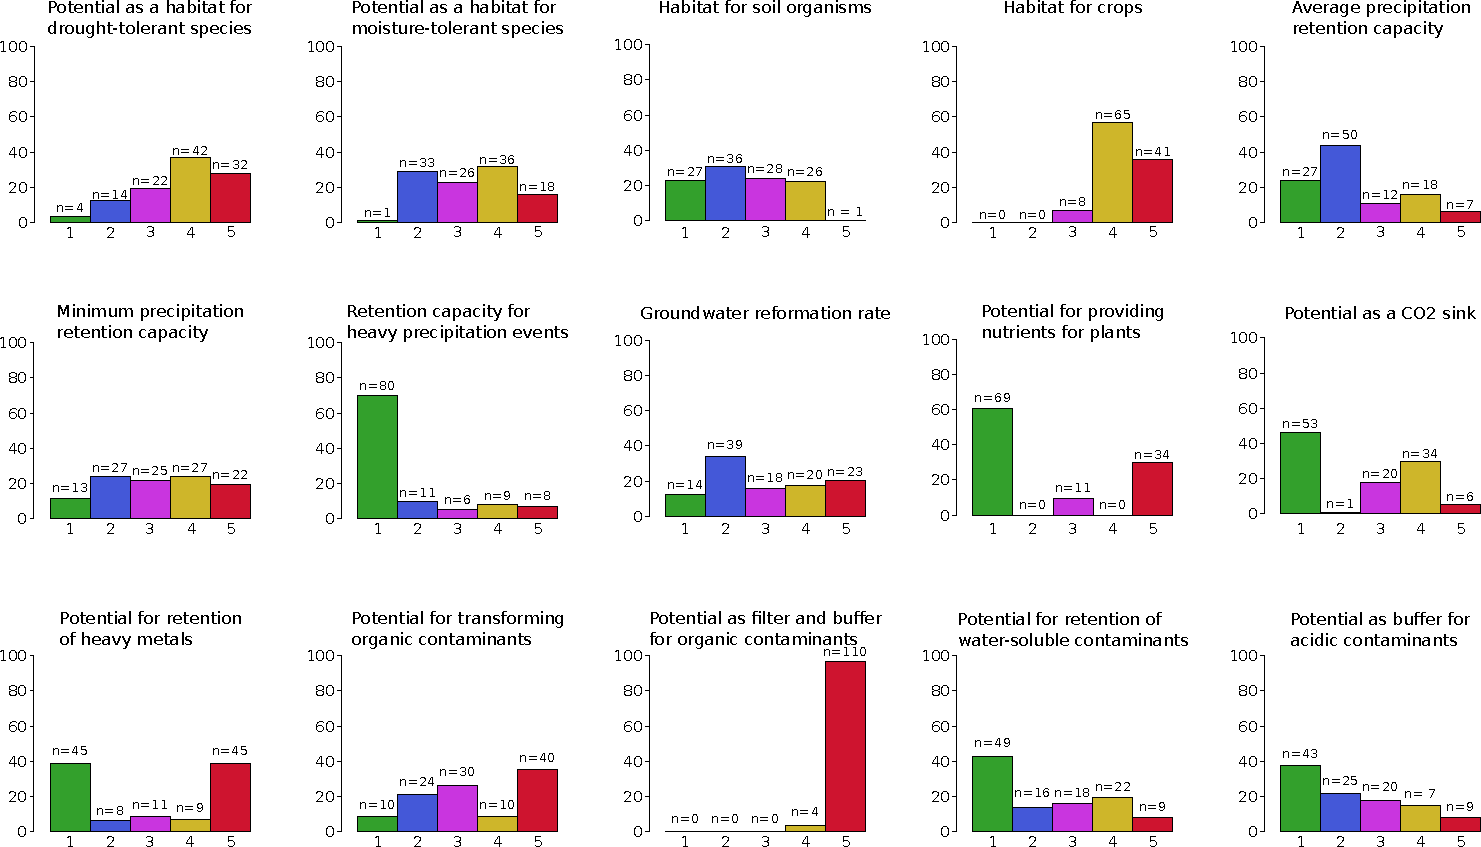
\includegraphics[width=\textwidth,angle=0]{soilfunctiondistro.pdf}
\caption{Barplots representing the distribution of the soil function grades for the various analysed potentials. }
\label{fig:SFdistro}
\end{figure}
A first evaluation of the feature selection procedure shows that mostly 2 parameters are sufficient, that is that there is no increase in cross-validated prediction accuracy  by adding more predictors, and most of the time these a combination of a landform classification and a local terrain parameter.
\begin{table}[!htbp]

\caption{Accuracy values (\%) and parameters for the different potentials}
\resizebox{0.95\textwidth}{!}{%
\centering
\tiny
\begin{tabular}{l|ccccc}
  \hline
  \hline
potential & parameter & res & windowsize & multiacc & testacc\\ 
  \hline
habitat for drought-tolerant species & landforms & 10 & 100 &  &\\ 
 & slope & 50 & 350 & 50.0 & 50.0\\ 
  \hline
habitat for moisture-tolerant species & long. curvature & 2.5 & 7.5 & &\\ 
 & landforms & 10 & 70 & 53.7 & 53.7\\ 
  \hline
habitat for soil organisms & cross-sec. curvature & 50 & 350 & & \\ 
 & slope & 50 & 350 &  &\\ 
 & convexity & 50 & 150 & 59.3 & 62.0\\ 
  \hline
agricultural production & slope & 2.5 & 7.5 & 86.1 & 86.1\\ 
  \hline
average precipitation retention capacity & cross-sec. curvature & 2.5 & 47.5 &  & \\
 & profile curvature & 10 & 150 & 50.9 & 54.6\\  
  \hline
minimum precipitation retention capacity & plan curvature & 2.5 & 72.5 &  & \\ 
 & minimal curvature & 50 & 150 & 41.6 &46.3\\ 
  \hline
retention capacity for heavy precipitation events & long. curvature & 10 & 150 & 73.1 & 73.1\\ 
  \hline
groundwater reformation rate & cross-sec. curvature & 2.5 &57.5 &  & \\ 
& profile curvature & 10 & 50 & 47.2 & 49.1\\
  \hline
providing nutrients for plants & minimal curvature & 2.5 & 22.5 & 71.3 & 72.2\\ 
  \hline
CO\textsubscript{2} sink & minimal curvature & 2.5 & 27.5 & 61.1 & 61.1\\ 
  \hline
retention of heavy metals & landforms & 10 & 70 & 63.9 & 63.9\\ 
  \hline
transforming organic contaminants & landforms & 10 & 500 & & \\ 
& maximal curvature & 10 & 70 & 46.3 & 50.0\\
  \hline
filter and buffer for organic contaminants & - & - & - & - &- \\ 
  \hline
 retention of water-soluble contaminants & slope & 2.5 & 27.5 &  & \\ 
 & minimal curvature & 2.5 & 7.5 &53.7 & 59.3\\ 
  \hline
buffer for acidic contaminants & plan curvature & 2.5 & 12.5 & & \\ 
 & slope &2.5 & 12.5  & 48.1 & 50.0\\ 
  \hline

\end{tabular}}
\label{table:cvacc}
\end{table}
\subsection{Potential as a habitat for drought-tolerant species}
Figure~\ref{fig:SFdistro} shows that of the 108 soil profile sites in the study area, 38 fall into class 4 (35\%) and 32 into class 5 regarding the potential as a habitat for drought-tolerant species. The intermediate class 3 contains 21 soil profiles whereas the high potential classes 1 and 2 are attribute to only 4 and 13 sites, respectively. 
As the predictor set does not contain landuse nor soil type, the SVM classification essentially attempts to model the different classes of available field capacity. In the majority of the feature selection runs a landform map based on a flatness threshold between 3 and 5$^{\circ}$,a spatial resolution of 10~m and a search radius of 100~m was chosen as the first predictive feature. The landform flat is dominant amongst the profile sites with a graded potential of 5, which is accordingly connected to minimal curvature values around 0. The landform slope is  most common for profiles with a potential  of 4, whereas spurs and hollow can present profile locations with a  potential score of 2 and, as expected, have increasingly negative minimum curvature values. A support vector classifier using theselandforms and slope at a low DTM resolution as predictor variables, results in a median cross-validated prediction accuracy of 50\%, where the most common error is that  a large number of sites are mistakenly classified as having grade 4. Nevertheless, the general implications of the feature selection are plausible, as flat areas  can  be expected to have higher field capacity values than sloping regions with negative curvature values.
\subsection{Potential as a habitat for moisture-tolerant species}
Only one soil profile site in the study area is awarded the best grade (1) for its potential as a habitat for moisture-tolerant species. As seen in Figure~\ref{fig:SFdistro}, the intermediate classes (two to four) are quite equally distributed with 33, 26 and 36 members, respectively. The class with the poorest potential consists of 18 soil profile sites.  Given the similarity in soil parameters and profile site characteristics used for the evaluation of this potential and the potential as a habitat for drought-tolerant species, a very similar landform classification  is chosen in the feature selection procedure (Table~\ref{table:cvacc}). This feature is complemented by the local terrain parameter longitudinal curvature to achieve the best median cross-validated accuracy  of 53.7\% with a SVM-model of this potential. The model shows that while the good grades are associated with
\section{Conclusion}
 

\section*{Acknowledgements} This research was performed within the project 'Terrain Classification of ALS Data to support Digital Soil Mapping', funded by the Autonomous Province Bolzano -- South Tyrol (15/40.3).

\section*{References}
\bibliography{P3.bib}

\end{document}
